%===================================== CHAP 4 =================================

\chapter{Requirements engineering}
\label{ch:requirements_engineering}

\section{Requirements description}

The requirements engineering process was a continuous negotiation between the customer and the development team. Although the customer had a general idea of what the system was supposed to do, this process went on throughout the duration of the project. This was done to make sure that the requirements were realistic, given the time available. The requirements lists reflect the final result of the process.

Requirements are separated into two categories. A functional requirement describes a function of the system or one of its components. A non-functional requirement can be viewed with regards to the operation of the system. Rather than listing specific functions of the system, it describes the performance or operation of the system as a whole. In this project, strict requirements and narrow requirement scope was not provided by the customer. The requirements given were general, and listed some features the system would have to provide, but not an extensive list. This led to the group having to create a more comprehensive set of requirements as a basis for development.

For the remainder of this chapter, a client is defined as any application that implements the protocol in question as its means of communication. Implementing a general purpose client was not a part of the product description. To the best of the groups knowledge, only one general purpose client exists for the protocol versions implemented. And it is a commercial client supporting AMQP 1.0. As such, libraries and scripts were used internally as client representations. These are covered in appendix \ref{sec:test_clients}.

\section{Requirements elicitation}
\label{sec:requirements_engineering-requirements_elicitation}

The functional requirements were elicited as a result of discussion both within the group and with the customer. Additional requirements were taken into consideration from the results of the research phase, as well as from the standards of WSN, AMQP and MQTT. Use cases and user stories were used as support tools for the group to define the exact requirements and formulations of them. This was due to the lack of strictly defined requirements from the customer. The use cases describe the steps that are needed to be performed in order to accomplish a certain task. The result of the process was a list, describing the requirements and the prioritization of them.

The non-functional requirements elicitation was purely a result of discussion with the customer. After identifying the properties of the system, they were classified and rated in order of importance.

Two issues arose when requirements for the different protocols were to be defined. First of all, the customer wanted as many protocols to be implemented as possible. After considering the time available, the three most important protocols were listed as requirements. The decision was subject to change however, depending on how much time it would take to implement each protocol.

The other issue was defining the protocols as requirements. On the one hand, they could be seen as functional requirements. "As a user, one must be able to send a message using protocol A". This would be regarded as a functional requirement. On the other hand, protocol support could be viewed as a property of the system. The protocol would then be considered a set of standards the system has to conform to, and fall under the compatibility category of non-functional requirements. The functional requirements would then only be described as "a user being able to send a message", regardless of protocol. The decision would not make any profound difference to the product. Thus, extensive research into this definition was not pursued.

\section{Functional requirements}
\label{sec:requirements_engineering-functional_requirements}

After a brief evaluation, the aspects around different protocols were defined as functional requirements, noted as FR in the requirements table. Mainly due to a consideration of how they would be tested. It seemed more reasonable to include them as functional requirements when considering the integration testing of components, as well as system and acceptance testing. The other functional requirements were concerned with what a user was supposed to do with the user interface. The general goal of the interface was to expose configuration of mappings between supported protocols, publisher and subscriber database listings, as well as topics and content filters. The functional requirements are described in table \ref{tab:func-requirements}, and was a result of the requirements elicitation process.

\begin{longtable}{@{\extracolsep{\fill}}|l|l|p{8cm}|l|@{}}
\hline
\rowcolor{lightgray}
\multicolumn{4}{|c|}{\textbf{Functional requirements}}  \\ \hline
\multicolumn{1}{|c|}{\textbf{$\#$}} & \textbf{Use Case} & \textbf{Description}    & \textbf{Priority} \\ \hline
\multicolumn{1}{|c|}{FR1} & \multicolumn{1}{c|}{U5, U6} & A user must be able to send and receive messages over the WSN protocol, with a client of his/her choice. & 
\multicolumn{1}{c|}{1} \\ \hline
\multicolumn{1}{|c|}{FR2} & \multicolumn{1}{c|}{U7} & A user must be able to subscribe to a topic using the WSN protocol, with a client of his/her choice. &
\multicolumn{1}{c|}{1} \\ \hline
\multicolumn{1}{|c|}{FR3} & \multicolumn{1}{c|}{U8} & A user must be able to register as a publisher on a topic using the WSN protocol, with a client of his/her choice. &
\multicolumn{1}{c|}{1} \\ \hline
\multicolumn{1}{|c|}{FR4} & \multicolumn{1}{c|}{U9} & A user must be able to unsubscribe from a topic using the WSN protocol, with a client of his/her choice. &
\multicolumn{1}{c|}{1} \\ \hline
\multicolumn{1}{|c|}{FR5} & \multicolumn{1}{c|}{U10} & A user must be able to unregister as a publisher on a topic using the WSN protocol, with a client of his/her choice &
\multicolumn{1}{c|}{1} \\ \hline
\multicolumn{1}{|c|}{FR6} & \multicolumn{1}{c|}{U11} & A user must be able to retrieve the latest message on a topic using the GetCurrentMessage function, using the WSN protocol, with a client of his/her choice. &
\multicolumn{1}{c|}{1} \\ \hline
\multicolumn{1}{|c|}{FR7} & \multicolumn{1}{c|}{U12} & A user must be able to renew his/her subscription using the WSN protocol, with a client of his/her choice. &
\multicolumn{1}{c|}{1} \\ \hline
\multicolumn{1}{|c|}{FR8} & \multicolumn{1}{c|}{U13} & A user must be able to pause his/her subscription using the WSN protocol, with a client of his/her choice. &
\multicolumn{1}{c|}{1} \\ \hline
\multicolumn{1}{|c|}{FR9} & \multicolumn{1}{c|}{U14} & A user must be able to resume his/her subscription using the WSN protocol, with a client of his/her choice &
\multicolumn{1}{c|}{1} \\ \hline
\multicolumn{1}{|c|}{FR10} & \multicolumn{1}{c|}{U15} & A user must be able to send multiple notification messages in a single Notify using the WSN protocol, with a client of his/her choice. &
\multicolumn{1}{c|}{1} \\ \hline
\multicolumn{1}{|c|}{FR11} & \multicolumn{1}{c|}{U5 \& U6} & A user must be able to send and receive messages using the AMQP protocol, with a client of his/her choice. &
\multicolumn{1}{c|}{1} \\ \hline
\multicolumn{1}{|c|}{FR12} & \multicolumn{1}{c|}{U16} & A user must be able to subscribe to a topic using the AMQP protocol, with a client of his/her choice. &
\multicolumn{1}{c|}{1} \\ \hline
\multicolumn{1}{|c|}{FR13} & \multicolumn{1}{c|}{U17} & A user must be able to unsubscribe using the AMQP protocol, with a client of his/her choice. &
\multicolumn{1}{c|}{1} \\ \hline
\multicolumn{1}{|c|}{FR14} & \multicolumn{1}{c|}{U1} & An administrator must be able to map topics/dialects with other topics. &
\multicolumn{1}{c|}{2} \\ \hline
\multicolumn{1}{|c|}{FR15} & \multicolumn{1}{c|}{U2} & An administrator must be able to edit the different subscriptions. That means delete one or all subscriptions on a given topic. This also includes deleting all topics. & \multicolumn{1}{c|}{3} \\ \hline
\multicolumn{1}{|c|}{FR16} & \multicolumn{1}{c|}{U  3} & An administrator must be able to get information in the administrator interface about the server. &  \multicolumn{1}{c|}{4} \\ \hline
\multicolumn{1}{|c|}{FR17} & \multicolumn{1}{c|}{U4} & An administrator must be able to log in with a user name and password to get access to core functions. & \multicolumn{1}{c|}{5} \\ \hline
\caption{Functional requirements}
\label{tab:func-requirements}
\end{longtable}

\clearpage

\section{Non-functional requirements}
\label{sec:requirements_engineering-non_functional_requirements}

Following is a list of the non-functional requirements (hereby denoted NFR) created. The requirements are listed in descending order of importance. 

\subsection{NFR1 - Extendability}
\label{subsec:requirements_engineering-non_functional_requirements-extendibility}

\subsubsection{NFR1.1 - Modularization}
\label{subsec:requirements_engineering-non_functional_requirements-modularization}

The different components of the system should be decomposed in such a way that the respective components are loosely coupled, to allow easier addition of more protocols at a later point in time. It also allows upgrading and further developing of different parts of the system individually.

\subsubsection{NFR1.2 - Protocol Independence}
\label{subsec:requirements_engineering-non_functional_requirements-protocol_independence}

The system must be able to translate between protocols independent of their type, more precisely it must not only support to/from WSN, but also between other supported protocols, without having to go through WSN.

\subsection{NFR2 - Documentation}
\label{subsec:requirements_engineering-non_functional_requirements-documentation}

All parts of the application must be documented according to the language specific standards, preferably in English.

\subsection{NFR3 - Open Source}
\label{subsec:requirements_engineering-non_functional_requirements-open_source}

The software shall be open source. The software shall be available for use, change and distribution by anyone. It will be licenced under the MIT license \cite{mit-license}. The code will remain available on Github after completion.

\section{User stories}
\label{sec:requirements_engineering-user_stories}

The following table describes the user stories defined. The stories were used as a tool to create use cases. The stories were defined based on conversations with the customer, and answers to what the customer wanted to do with the system. The different aspects were then structured in table \ref{tab:user-stories}. 

\clearpage

\begin{longtable}{@{\extracolsep{\fill}}|l|p{5cm}|p{5cm}|@{}}
\hline
\rowcolor{lightgray}
\multicolumn{3}{|c|}{\textbf{User stories}} \\ \hline
\textbf{As a(n)} & \textbf{I want to} & \textbf{So that (I can)}  \\ \hline
Admin & Log in with username and password. & Gain access to the system. \\ \hline
Admin & Get information about server. & See number of subscribers and system status.  \\ \hline
Admin & Get information about subscribers. & See number of connections to the broker.  \\ \hline
Admin & Get server information. & See which IP the broker is running on. \\ \hline
Admin & Get IP and topics information. & See information about subscribers and topics. \\ \hline
Admin & Get resource overview. & See load and balance of the server. \\ \hline
Admin & Edit topics/dialects. & Map topics/dialects. \\ \hline
Admin & Edit subscriptions. & Unsubscribe users on topics. \\ \hline
Admin & Edit topics. & Delete a topic. \\ \hline
Client & Subscribe with AMQP or WSN & receive messages. \\ \hline
Client & Register as publisher with AMQP or WSN & send messages. \\ \hline
Client & Unsubscribe & No longer receive messages. \\ \hline
Client & Unregister & No longer send messages. \\ \hline
\caption{User stories}
\label{tab:user-stories}
\end{longtable}

\clearpage

\section{Use cases}
\label{sub:requirements_engineering-use_cases}

The use-cases were mainly used for internal communication within the group, as a simple way to share information about the high-level workings of the system. They were also used as a tool to help create and visualize the requirements. Additionally, the group used the use cases to evolve and expand the administration interface by adding information that was useful during the creation of the use cases and the development phase. One use-case diagram is covered here as an example, the rest can be found in appendix \ref{sec:use_cases_appendix}.

\subsection{Use case 1 - Topic mapping}
\label{subsec:requirements_engineering-use_cases-topic_mapping}

After (and/or before) a publisher has added a topic, the admin must be able to map this topic to another topic. The topic mapping interface must also provide a way of creating a relay from messages received on one topic, to a different topic.

{\centering
\begin{table}[ht!]
\begin{minipage}{.5\textwidth}
\centering
\resizebox{\textwidth}{!}{
\begin{tabular}{|l|p{5cm}|}
\hline
\textbf{Use case ID} & U1 \\ \hline
\textbf{Use case Name} & Topic mapping \\ \hline
\textbf{Description} & Admin should be able to map between topics.  \\ \hline
\textbf{Pre conditions} & The admin is logged in.\\ \hline
\textbf{Standard flow} & \begin{enumerate}
\item Click the config pane.
\item Enter the topic you want to map from.
\item Enter the topic you want to map to.
\item Click the "Add"-button.
\end{enumerate} \\ \hline
\textbf{Alternative flow} & \begin{description}
\item[2A:] Server will not answer request  \begin{enumerate}
\item Display error message.
\item Open config file for topic mapping.
\item Edit file with the mapping.
\item Save config file.
\item Restart/reload server.
\end{enumerate}
\end{description} \\ \hline
\textbf{Post conditions} & Subscribers of different topics now receive a notify when a publisher publishes on one of the topics.  \\ \hline
\end{tabular}
}
\caption{Use case 1 - Topic mapping}
\end{minipage}
\hfill
\begin{minipage}{.4\textwidth}
\centering
\begin{center}
    \makebox[\textwidth]{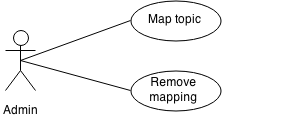
\includegraphics[width=\textwidth]{fig/usecase/usecase_v3_map.png}}
    \captionof{figure}{U1 - Topic mapping}
    \label{fig:u1}
\end{center}
\end{minipage}
\end{table}
}

\clearpage